\documentclass[10pt, a4paper]{article}
\usepackage[utf8]{inputenc}
\usepackage{amsrefs}
\usepackage{tikz, wasysym}
\usetikzlibrary{automata,positioning}
\usepackage[]{algorithm2e}
\usepackage[]{csquotes}

\author{Sven Fiergolla}
\title{Research Methods \& wissenschaftliches Arbeiten mit \LaTeX}
\date{\today}

%TODOs: fix empfy last page
%		fill placeholher

\begin{document}
\maketitle

\paragraph{Abstract}
Dies ist eine Zusammenfassung über die Enstehung von wissenschftlichen Arbeiten als solches, sowie den dabei notwendigen Einsatz von \LaTeX\  zur Ausarbeitung.
\par
\tableofcontents
\bigskip
%\pagebreak
%\chapter{Wissenschaftliche Arbeiten}

\section{Einführung}
\subsection{Gründe für die Publikaton}
\paragraph{}
Wissenschaftler haben verschiedene Beweggründe für die Veröffentlichung ihrer Resultate aus Forschung, Kongressen oder ähnlichem:
\par
\begin{itemize}
\item den Zeitpunkt einer Erkenntnis zu dokumentieren
\item die Ergebnisse der Arbeit zu teilen und sie zitierbar zu machen
\item sich im eigenen Fach einen Ruf zu verschaffen
\item Geld durch die Veröffentlichung zu erhalten \textit{(Tantieme)}
\item sich in der allgemeinen Öffentlichkeit bekannt zu machen
\end{itemize}
\par
\paragraph{}
Dazu verfassen sie sogenannte \enquote{Paper}, eine strukturierte Verschriftlichung der Resultate als wissenschaftliche Arbeit, zur Veröffentlichung.
\par

\subsection{Aufbau einer Arbeit}
\paragraph{}
Der grundsätzliche Aufbau einer wissenschaflichen Arbeit umfasst:
\begin{itemize}
\item den Titel, die Authoren und andere übergeordnete Informationen (Affiliation, Datum etc.)
\item ein Abstract (eine allgemeine Zusammenfassung)
\item eine Einführung mit den Grundlagen der Fragestellung
\item Ablauf der Forschung/Konferenz
\item technische Details/Beweis der Resultate
\item Conclusion (Fazit) und zukünftige Aspekte
\item References (Literaturverzeichnis)
\item Author Contributions () und Conflict of Interests ()
\end{itemize}
\par

\paragraph{}



\section{Wissenschaftliche Arbeiten}
\subsection{Die \textit{DBLP}}
1

\subsection{Research Methods}
2

\subsection{TCS Magazin}
%TODO
3

\subsection{Google Scholar}
\paragraph{}
Das zunehmend an Bedeutung gewinnende \textit{Google Scholar} dient als öffentliche Suchmaschine für wissenschaftliche Arbeiten und andere Veröffentlichungen. Zudem ist sichtbar, wie häufig ein Paper von anderen zitiert wurde.
\par
%TODO: insert picture


\subsection{Der \textit{Ipact-Factor}}




%\chapter{\LaTeX}
\section{Funktionalität von \LaTeX}
\subsection{Allgemeine Funktionalität}

\subsection{Vorteile gegenüber \textit{WYSIWYG-Editoren}}
\subsection{Graphen}
\paragraph{}
1.Graph


	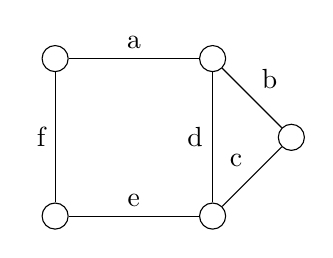
\begin{tikzpicture}[node distance=5cm,on grid,auto]
   
   \node[shape=circle,draw=black] (1) at (0,0) {};
   \node[shape=circle,draw=black] (2) at (0,2) {};
   \node[shape=circle,draw=black] (3) at (2,0) {};
   \node[shape=circle,draw=black] (4) at (2,2) {};
   \node[shape=circle,draw=black] (5) at (3,1) {};
   

    \path[-] (1) edge node {f} (2);
    \path[-] (2) edge node {a} (4);
    \path[-] (3) edge node {d} (4);
   	\path[-] (4) edge node {b} (5);
   	\path[-] (3) edge node {c} (5);
	\path[-] (1) edge node {e} (3);
	
	\end{tikzpicture}
\par
\paragraph{}
2.Graph
	

	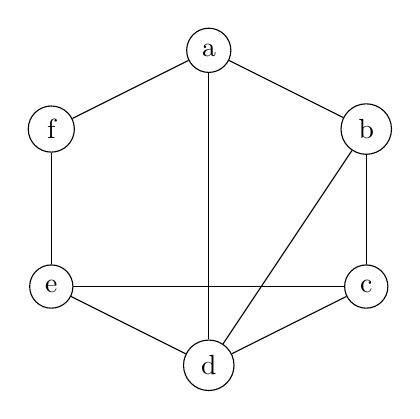
\begin{tikzpicture}[align=center, node distance=8cm,on grid]
   
   \node[shape=circle,draw=black] (1) at (0,0) {e};
   \node[shape=circle,draw=black] (2) at (0,2) {f};
   \node[shape=circle,draw=black] (3) at (4,0) {c};
   \node[shape=circle,draw=black] (4) at (4,2) {b};
   \node[shape=circle,draw=black] (5) at (2,3) {a};
   \node[shape=circle,draw=black] (6) at (2,-1) {d};
   

    \path[-] (1) edge node {} (2);
    \path[-] (2) edge node {} (5);
    \path[-] (3) edge node {} (4);
   	\path[-] (6) edge node {} (5);
   	\path[-] (4) edge node {} (5);
	\path[-] (1) edge node {} (3);
	\path[-] (1) edge node {} (6);
	\path[-] (3) edge node {} (6);
	\path[-] (4) edge node {} (6);
	
	\end{tikzpicture}
\par
\subsection{Pseudocode}
\paragraph{}
\begin{algorithm}[H]

 $q:=q_0$\\
 \For{$j:=1$ \KwTo $n$}{
 \While{$g[q,s_j]=$fail}{
  $q:=h[q]$\\}
  \If{q is in F}{\KwRet{\enquote{yes}}

   
 }

 }
  \KwRet{\enquote{no}}
 \par
 \bigskip
 
 \paragraph{}
 \caption{Fig. 9. The Aho-Corasik algorithm for matching multiple keywords}

\par
\end{algorithm}
%TODO:fix empty last page
\end{document}
